	\pagestyle{fancy}

	\section{Experimentelle Untersuchungen} \label{sec:Experimentelle Untersuchungen}

	\subsection{Versuchsziel und -planung}\label{sec:Versuchsziel und -planung}
	
	Der Hauptzweck dieses Experiments besteht darin, die Modalanalyse der HSC-Werkzeugschäfte unter Rotation und Exzentrizität durchzuführen. Dafür wurden folgende Teilaufgaben bearbeitet:
	
	\begin{enumerate}
		\item Äquivalente Realisierung der Rotation mit Exzentrizität bei HSC-Schäften.
		\item Festlegung geeigneter Versuchsobjekte (Abmessungen der Probekörper).
		\item Aufbau des Versuchsstands und Durchführung der Messungen.
	\end{enumerate}
	
	Die Messdaten sollen zum Validieren des theoretisch Modells eines rotierenden Schafts mit Exzentrizität dienen. Die Planung kann unterteilt werden in den allgemeinen Messaufbau und die Wahl der Probekörper.
	\\
	Für die Modalanalyse wird zur Erregung ein Impulshammer verwendet. Anschließend wird mit einem Beschleunigungssensor die Antwort gemessen und die Übertragungsfunktion ermittelt. Die Übertragungsfunktion ist mit
	

	
	\begin{equation}\label{equ:Übertragungsfunktion}
	H(\omega)\equiv \dfrac{Y(\omega)}{X(\omega)}
	\end{equation}
	
	gegeben un repräsentiert das komplexe Verhältnis zwischen Ausgang $ Y(\omega) $ und Eingang $ X(\omega) $ als Funktion der	(Kreis-) Frequenz $ \omega $. Die Übertragungsfunktion beschreibt die dynamischen Verhältnisse eines Systems unabhängig von der zur Messung benutzten Signalart \cite{dossing1989strukturen}.\\
	 
	Die Übertragungsfunktion wird dabei für verschiedene Anregungspunkte bestimmt. Diese Versuchsmethode erlaubt es nicht, die experimentelle Modalanalyse unter Rotation durchzuführen, da der Beschleunigungssensor kabelgebunden ist. Aus diesem Grund wird am oberen Ende des Werkzeugschafts eine Radialkraft angebracht. Damit wird die Wirkung der Fliehkraft infolge der Rotation sowie Exzentrizität äquivalent berücksichtigt. Durch die Formänderungsenergie kann der Zusammenhang zwischen die Radialkraft $ F $ und Schwerpunktgeschwindigkeit ($e \Omega$) bestimmt werden. Nach \cite{gross2017technische} lautet die Formänderungsenergie für einen Biegebalken 
	
	\begin{equation}\label{equ:Formanderungsenergie}
	W = \dfrac{1}{2} \int_{0}^{L} \dfrac{M_{b}^{2}(x)}{EI} \dx .
	\end{equation}
	
	Wie die Abbildung \ref{fig:Zusammenhang_Omega_F} gezeigt, für einen Balken mit Rotation und Exzentrizität ergibt sich das Schnittmoment zu
	
	\begin{equation}\label{equ:Biegemoment-Rotation}
	M_{b1}(x) = -\int_{x}^{L} \rho A e \Omega^{2} (\xi-x) \dxi = \rho A e \Omega^{2} \left[ -\dfrac{L^{2}}{2}+Lx-\dfrac{x^{2}}{2}\right] ,
	\end{equation}
	
	womit die Formänderungsenergie wie folgt
	
	\begin{equation}\label{equ:Formanderungsenergie-Rotation}
	W_{1} = \dfrac{1}{2} \int_{0}^{L} \dfrac{M_{b1}^{2}(x)}{EI} \dx = \dfrac{\rho^{2}A^{2}e^{2}\Omega^{4}L^{5}}{40EI}
	\end{equation}
	
	lautet. Beim Balken mit Radialkraft ergibt sich das Schnittmoment zu
	
	\begin{equation}\label{equ:Biegemoment-Radialkraft}
	M_{b2}(x) = F\cdot(x-L)
	\end{equation}
	
	und damit die Formänderungsenergie zu
	
	\begin{equation}\label{equ:Formanderungsenergie-Radialkraft}
	W_{2} = \dfrac{1}{2} \int_{0}^{L} \dfrac{M_{b2}^{2}(x)}{EI} \dx = \dfrac{F^{2}L^{3}}{6EI}.
	\end{equation}
	
	Das Verhältnis zwischen Radialkraft $ F $ und Schwerpunktgeschwindigkeit ($e \Omega$) folgt aus
	\begin{equation}\label{equ:Verhältnis-Rotaion-und-Radialkraft}
	W_{1} \overset{!}{=} W_{2} \,\,\,\,\,\,\,\,\,\Rightarrow F = \pm \dfrac{1}{2} \sqrt{\dfrac{3}{5}} \rho A L e \Omega^{2}.
	\end{equation}
	
	\begin{figure}[H]
		\centering
		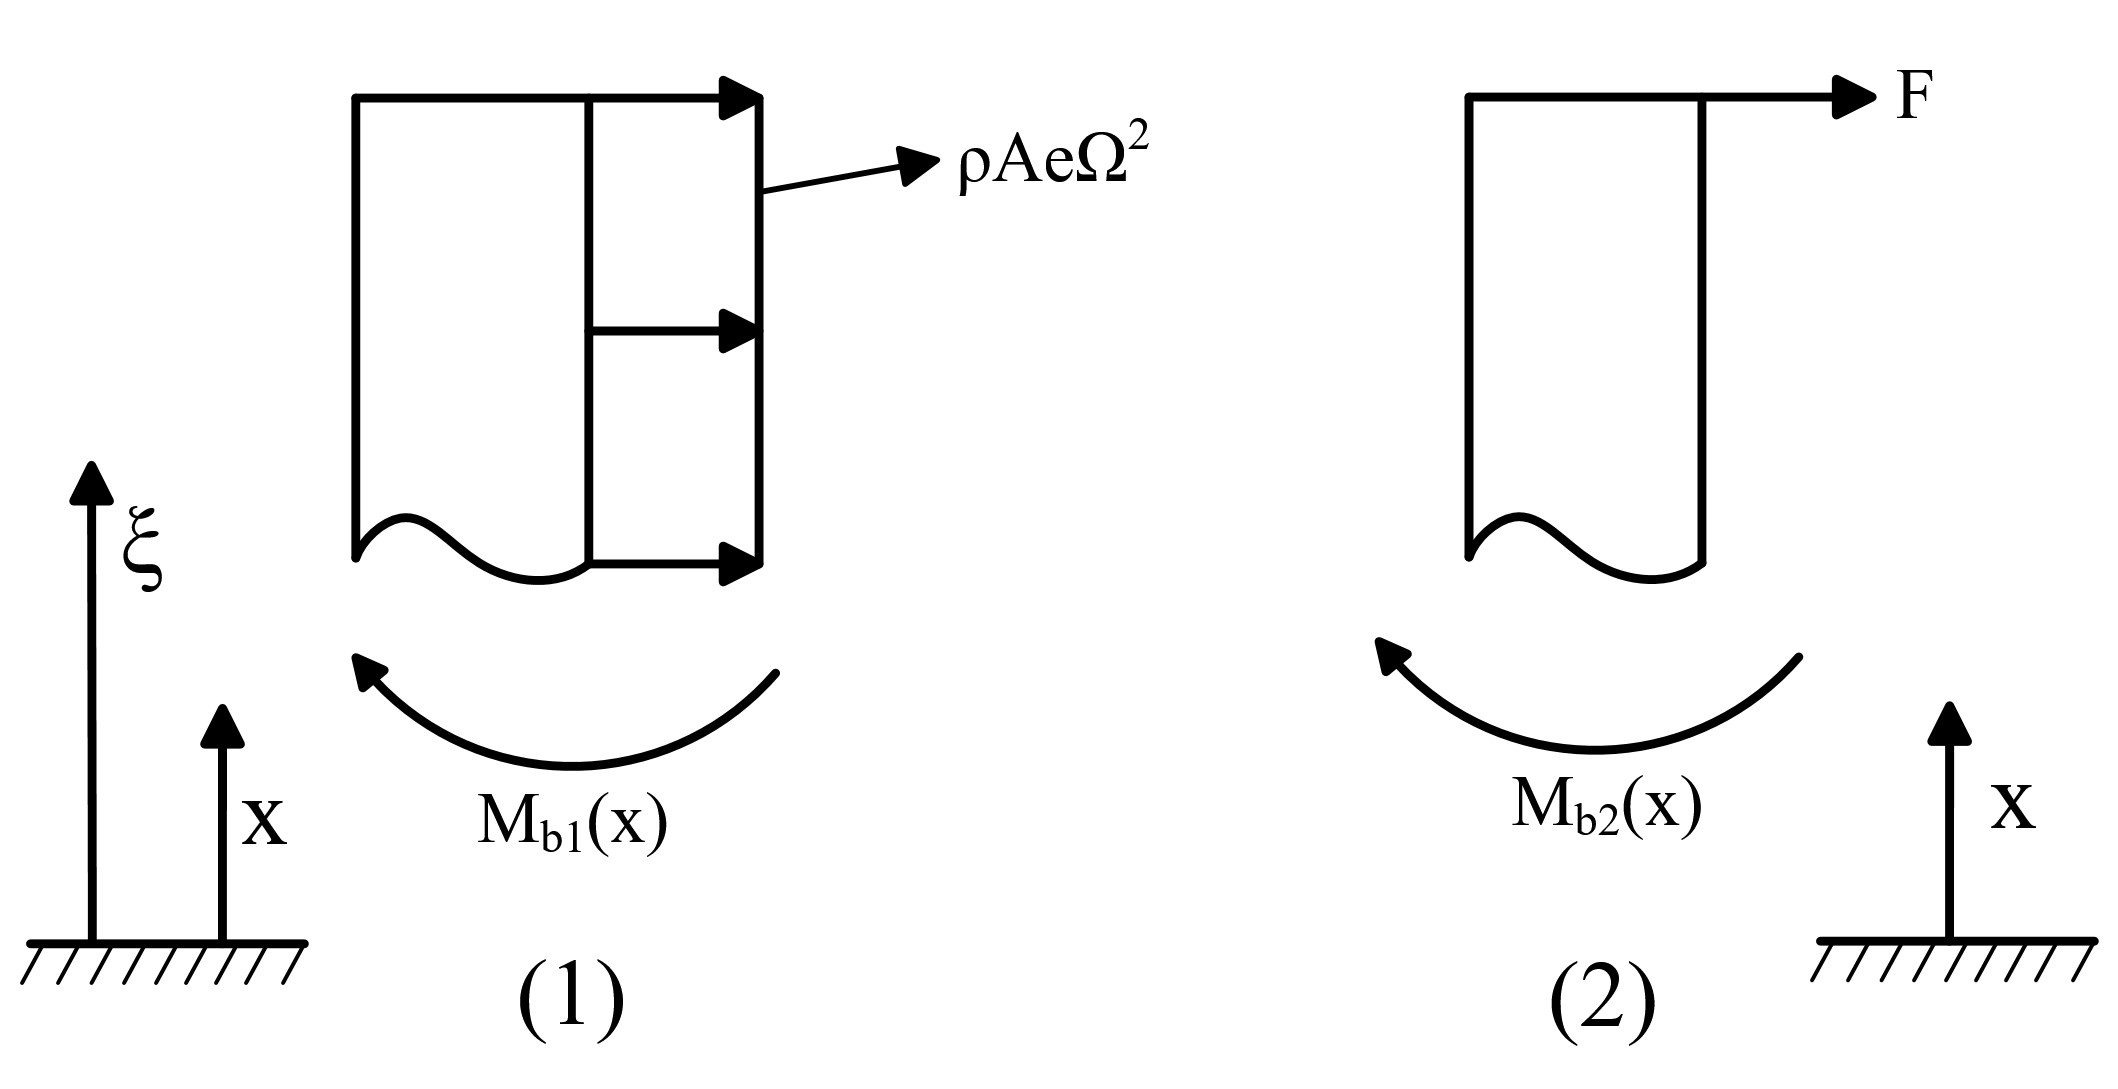
\includegraphics[width=0.85\linewidth, height=0.28\textheight]{Experimentelle_Untersuchungen/Zusammenhang_Omega_F}
		\caption{Schnittmoment für (1) einen Balken mit Rotation und Exzentrizität und (2) einen Balken mit Radialkraft.}
		\label{fig:Zusammenhang_Omega_F}
	\end{figure}
	
	Durch Änderung der Radialkraft können unterschiedliche Werte der Schwerpunktgeschwindigkeit ($e \Omega$) nach Gleichung \ref{equ:Verhältnis-Rotaion-und-Radialkraft} simuliert werden. Die Radialkraft soll dabei mit einer Feder aufgebracht werden, welche die Gesamtsteifigkeit möglichst wenig beeinflusst. Auf die Lagerung des Schaftes und die Verbindung mit der Feder wird später eingegangen \cite{Kokavecz2010}.
	
	\subsection{Versuchsaufbau}\label{sec:Versuchsaufbau}
	
	\subsubsection{Versuchsobjekt}\label{sec:Versuchsobjekt}
	Bei den Versuchen werden HSC-Hohlschäfte mit unterschiedlicher Wandstärke verwendet. Die dazugehörigen Parameter sind in der folgenden Tabelle \ref{tab:Datentabelle-Schaft} zusammengestellt.
	
	\begin{table}[H]\label{tab:Datentabelle-Schaft}
		%\renewcommand\arraystretch{1.2}
		\centering
		%\resizebox{\textwidth}{12mm}{		
		\begin{tabular}{|c|c|c|c|c|c|c|}
			\hline
		    Nr.     & Bezeichnung  & Werkstoff  & \makecell[c]{Aussen-\\durchmesser\\$  [mm] $}  & \makecell[c]{Wand-\\stärke\\$  [mm] $} & \makecell[c]{L/D-\\ Verhältnis} & \makecell[c]{Masse\\$  [g] $}\\
			\hline
		 	1       & Schaft-$ 10\times8 $     & S235J0   & 10          & 1      & 33       & 72,77 \\
			\hline
			2       & Schaft-$ 10\times9  $    & S235J0   & 10          & 0,5    & 33       & 38,41\\
			\hline	 
		\end{tabular}%}
		\caption{Parameter der verwendeten Versuchsschäfte.}
	\end{table}
		Für die Lagerung und Einbringung der Vorspannkraft ist es jedoch notwendig, weitere Bauteilen an den jeweiligen Schaft anzubringen. In Abbildung \ref{fig:Schaft-10x8} ist zunächst die Geometrie der Probe Nr.1 dargestellt. 
	
	\begin{figure}[H]
		\centering
		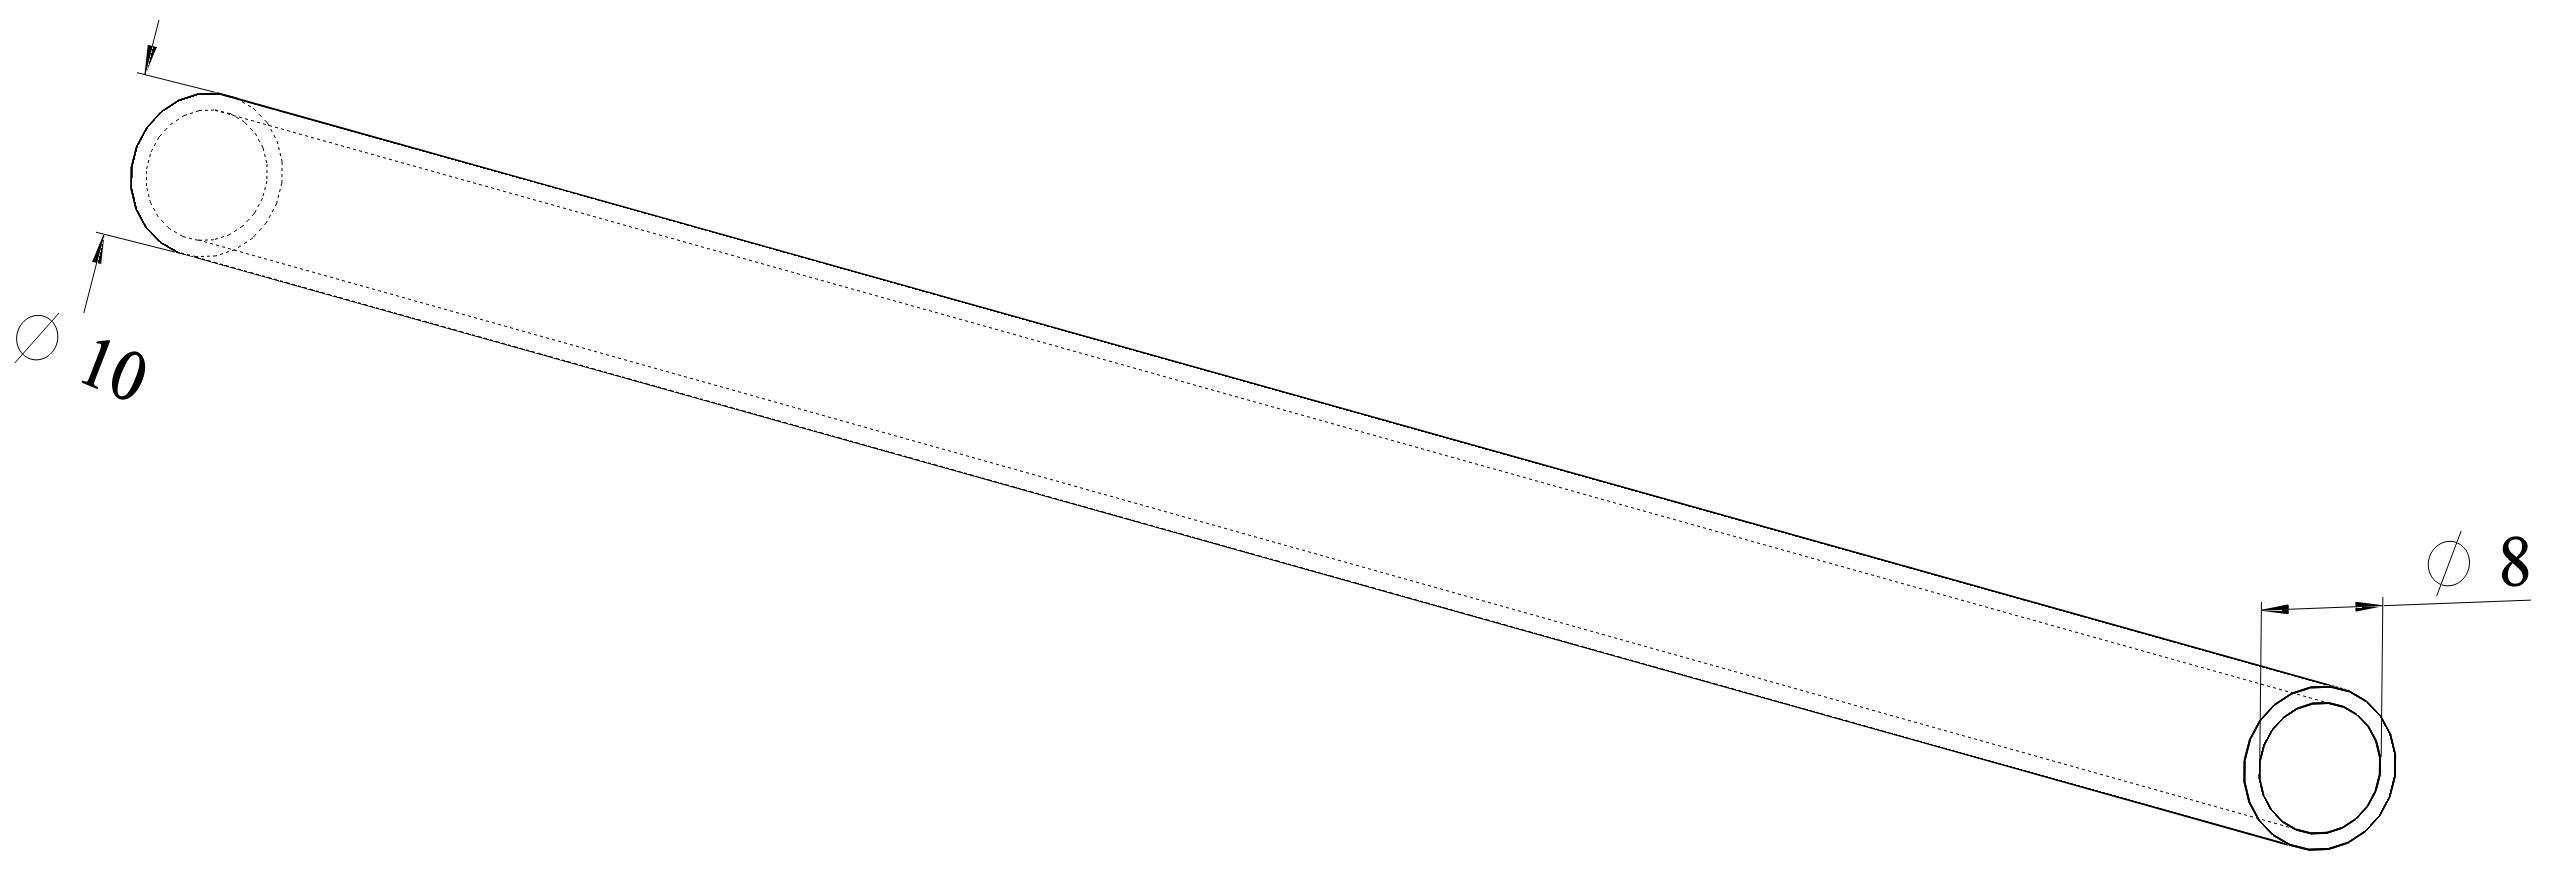
\includegraphics[width=0.9\linewidth, height=0.25\textheight]{Experimentelle_Untersuchungen/Schaft_10x8}
		\caption{3D-Modell von Probekörper Nr.1  (Schaft-$ 10\times8 $).}
		\label{fig:Schaft-10x8}
	\end{figure}

	Dazu wird das untere Ende des Schaftes auf einen Stopfen aufgeschrumpft. Analog dazu wird das obere Ende des Schaftes auf einen Stopfen für die Einbringung der Federkraft aufgeschrumpft. Die beiden Bauteile sind in Abbildung  \ref{fig:Stopfen-Schaft-10x8} dargestellt. \\
	
	Der Stopfen für die Krafteinbringung weist einen Würfeln am freien Ende auf. Dieser dient dazu, den Beschleunigungssensor magnetisch anzuheften. Weiterhin ist eine Gewindebohrung eingebracht, um eine Ringschraube einschrauben zu können. Über diese wird dann die Vorspannkraft mittels Feder eingeleitet. 
	
	
	
	
	\begin{figure}[H]
		\centering
		\begin{minipage}[t]{0.5\linewidth}
			\centering
			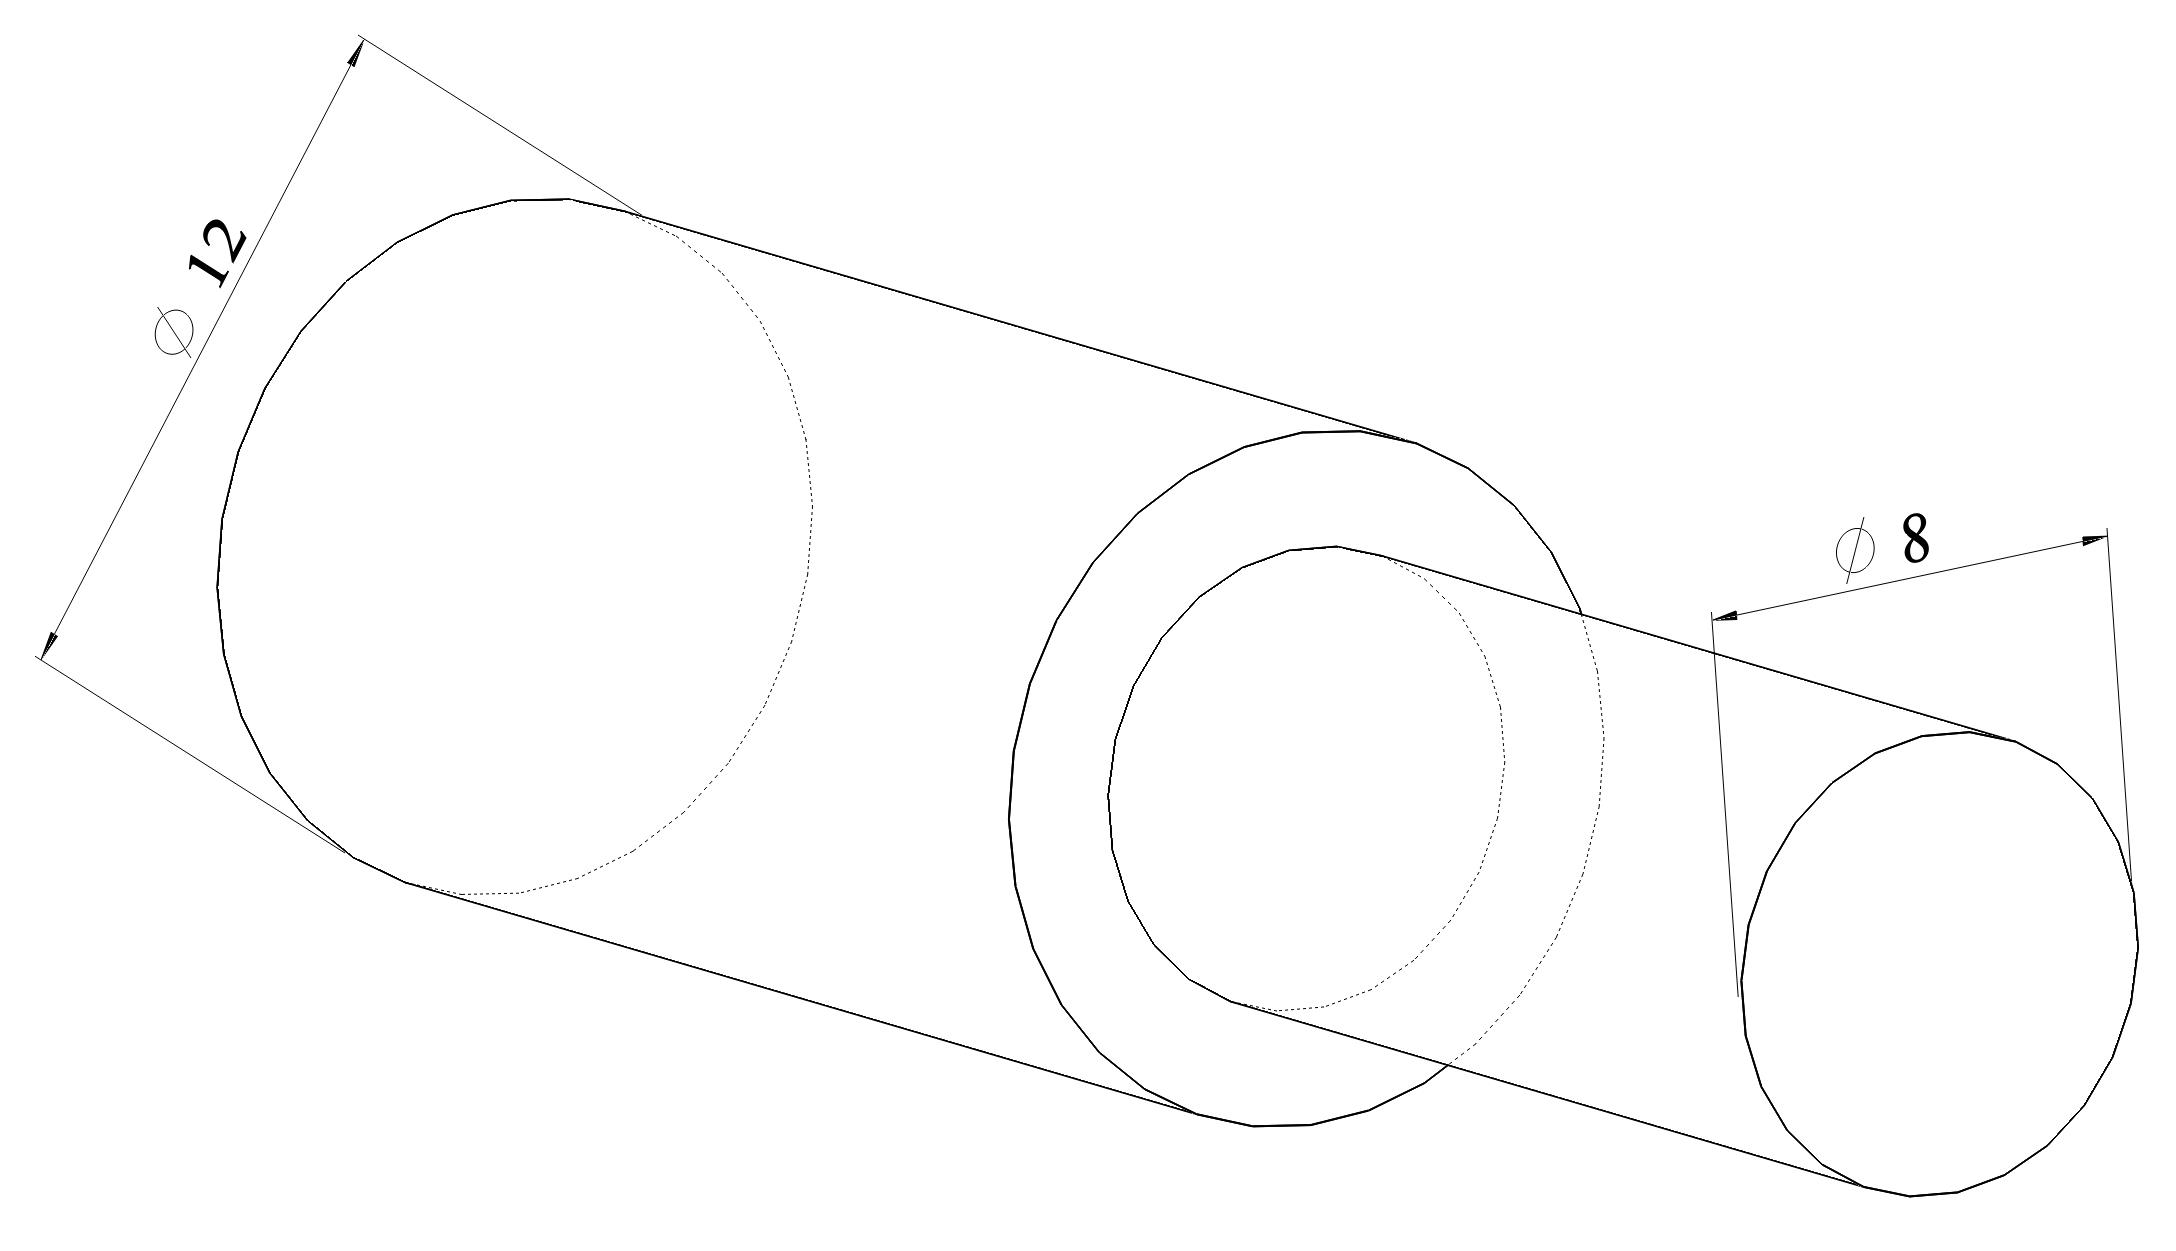
\includegraphics[width=1.0\linewidth, height=0.23\textheight]{Experimentelle_Untersuchungen/10x8_Lagerung_Stopfen}
		\end{minipage}% <- sonst wird hier ein Leerzeichen eingefügt
		\hfill
		\begin{minipage}[t]{0.45\linewidth}
			\centering
			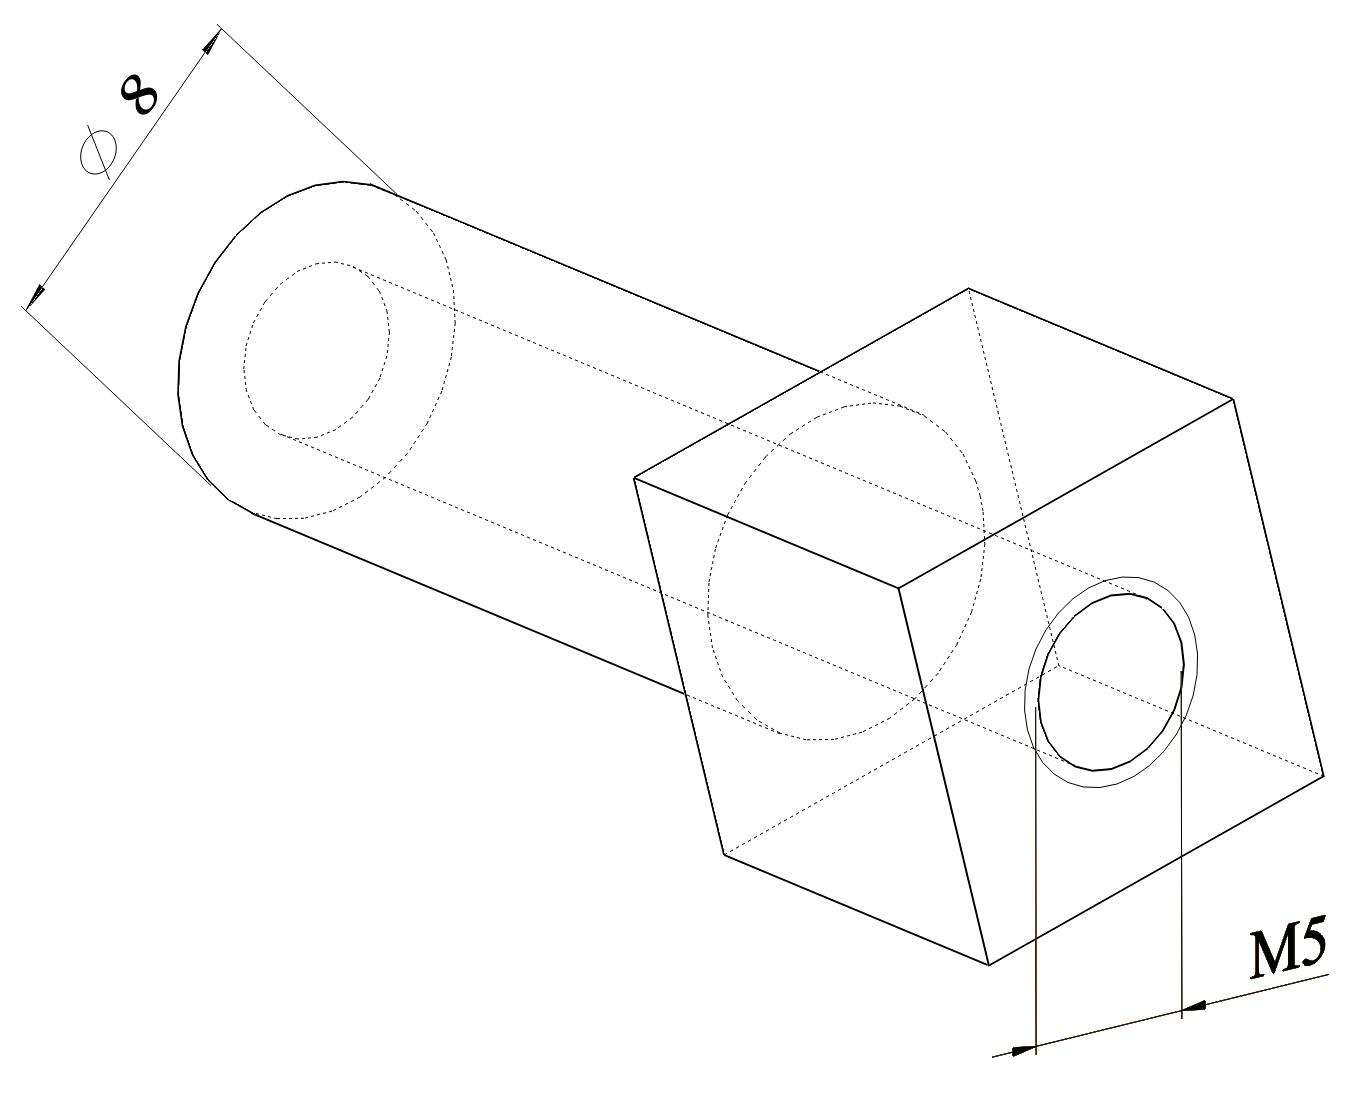
\includegraphics[width=1.0\linewidth, height=0.23\textheight]{Experimentelle_Untersuchungen/10x8_Schraube_Stopfen}
		\end{minipage}
	\caption{3D-Modelle der Stopfen für den Schaft-$ 10\times8 $ für die Lagerung (links) und Einbringung der Vorspannkraft (rechts).}
	\label{fig:Stopfen-Schaft-10x8}
	\end{figure}
	
	
	In Abbildung \ref{fig:Baugruppe-Schaft-10x8} ist nochmals der Zusammenbau der einzelnen Teile zu einer Baugruppe zu sehen. Darin ist auch eine Ringschraube enthalten, über welche die Feder zur Vorspannung eingehängt wird. Die komplette Bauteile (z.B. Aufnahmehaltung und -platte, Gegenkrafthaltung) sind durch die Zeichnungen im Anhang dargestellt.
	
	\begin{figure}[H]
		\centering
		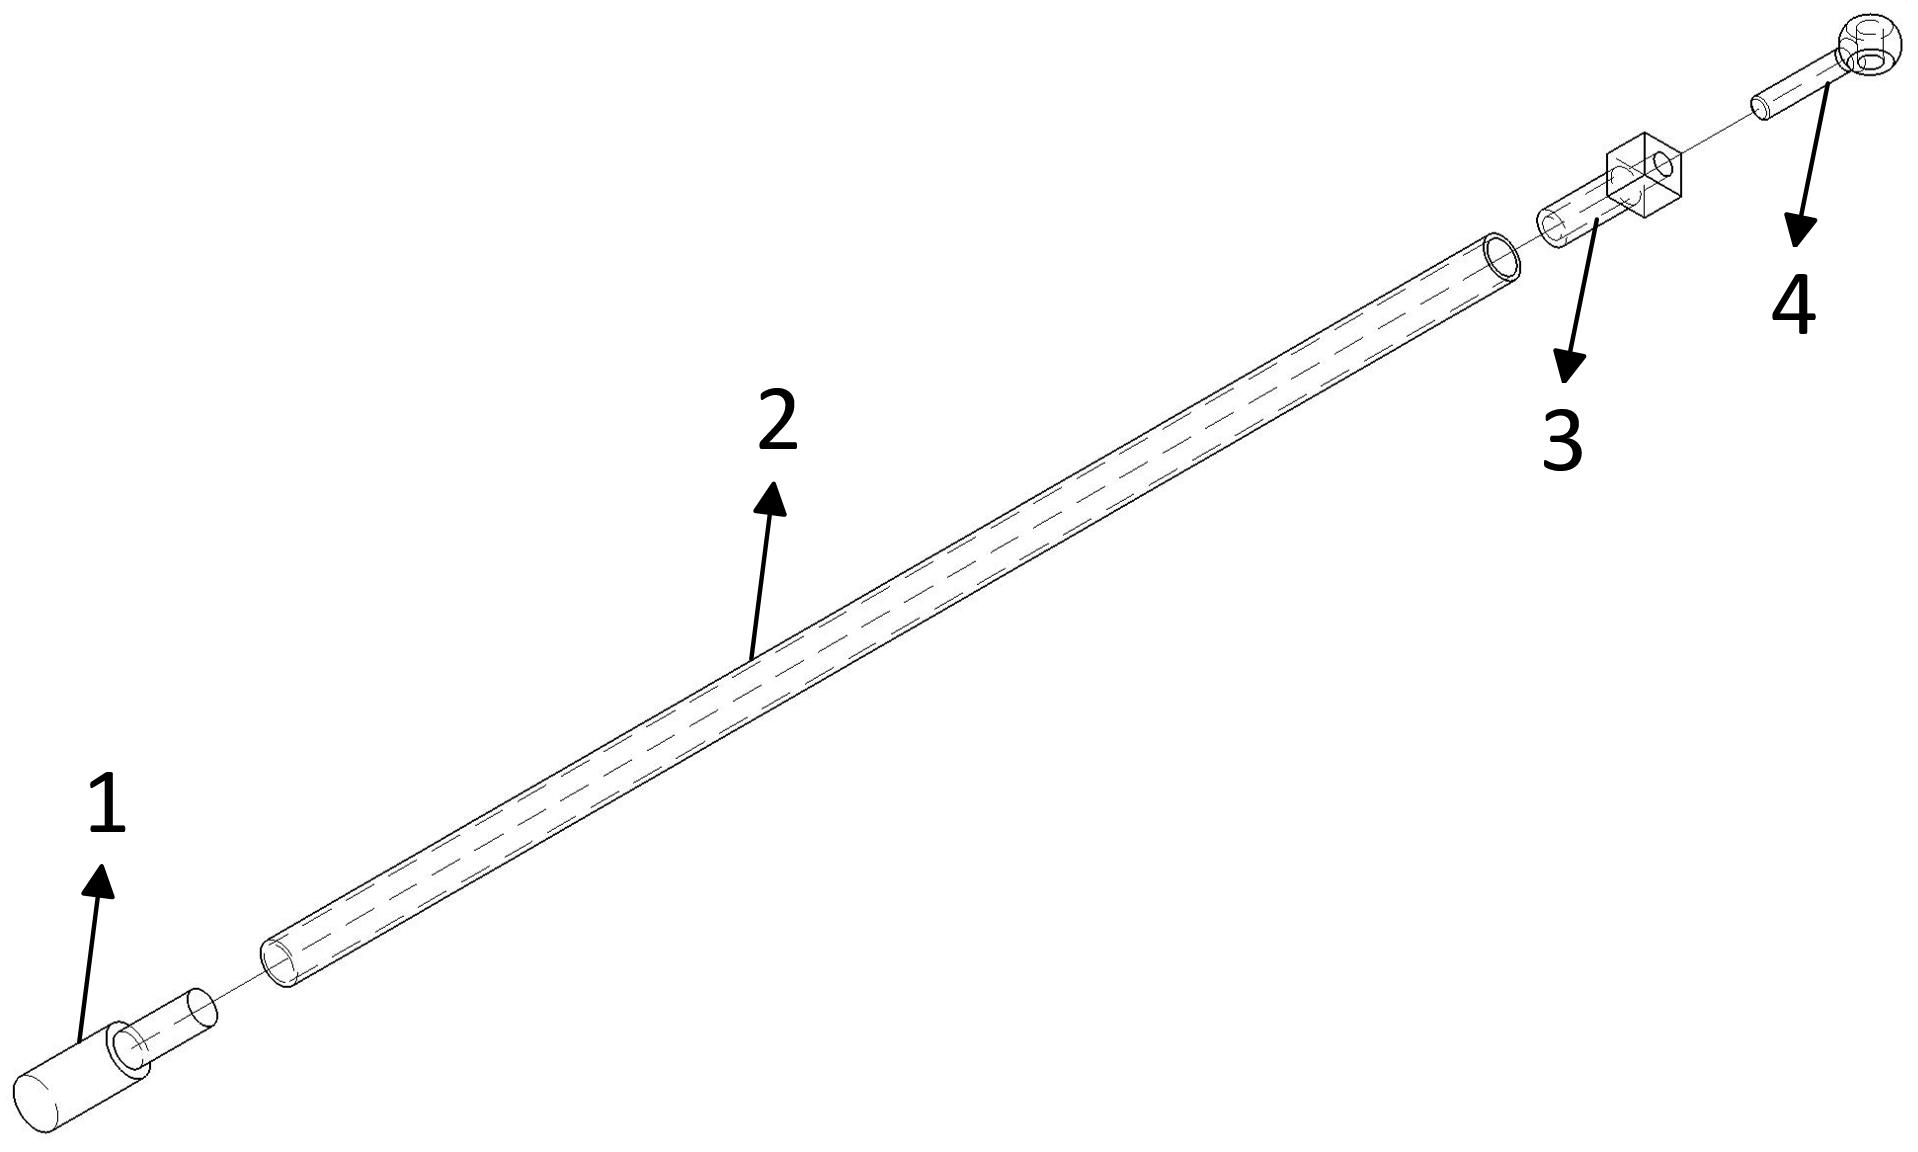
\includegraphics[width=0.85\linewidth, height=0.35\textheight]{Experimentelle_Untersuchungen/Schaft_10x8_Baugruppe}
		\caption{3D-Modell der Baugruppe des Schaftes-$ 10\times8 $ (1: Stopfen Lagerung, 2: Schaft, 3: Stopfen Vorspannkraft, 4: Ringschraube).}
		\label{fig:Baugruppe-Schaft-10x8}
	\end{figure}
	

	
	
	
	\subsubsection{Aufbau des Versuchsstandes}\label{sec:Aufbau des Versuchsstandes}
	
	Die Abbildung \ref{fig:Versuchsaufbau} zeigt die grundsätzlichen Komponenten des Versuchsaufbaus in der Prüfumgebung. Es handelt sich dabei um die folgende Objekte:
	\begin{itemize}
		\item Objekt 1: PC-Monitor mit der Bedienoberfläche von \textsc{PULSE LabShop}, um den Versuchsstatus zu überprüfen.
		\item Objekt 2: Impulshammer, welcher durch Anschlagen der Versuchsprobe die Anregung erzeugt.
		\item Objekt 3: Versuchskörper, wie er bereits in Abbildung \ref{fig:Baugruppe-Schaft-10x8} gezeigt wurde.
		\item Objekt 4: Beschleunigungssensor zur Messung Systemantwort.
		\item Objekt 5: Haltevorrichtung zur Befestigung der Feder.
		\item Objekt 6: Kraftsensor zur Messung der aufgebrachten Vorspannkraft.
		\item Objekt 7: Analog-Digital-Wandler, welcher die aktuelle Vorspannkraft anzeigt.
	\end{itemize}
	
	\begin{figure}[H]
		\centering
		\subfigure{ 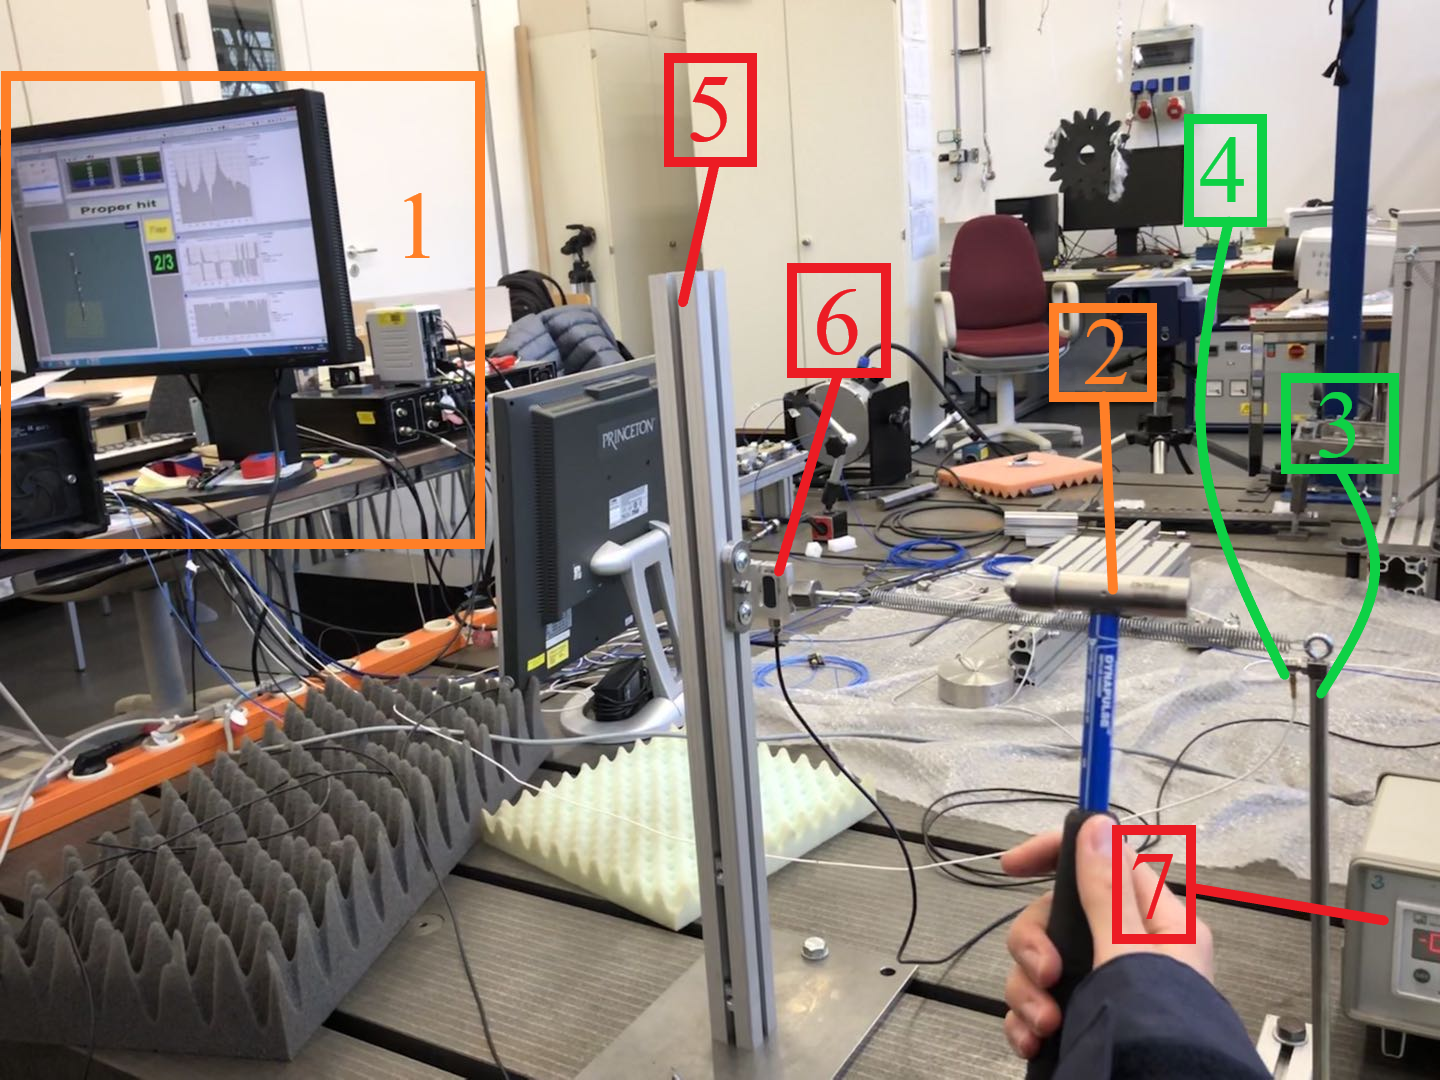
\includegraphics[width=0.48\linewidth, height=0.25\textheight]{Experimentelle_Untersuchungen/Aufbau_Versuchsstand_01.png} }
		\subfigure{ 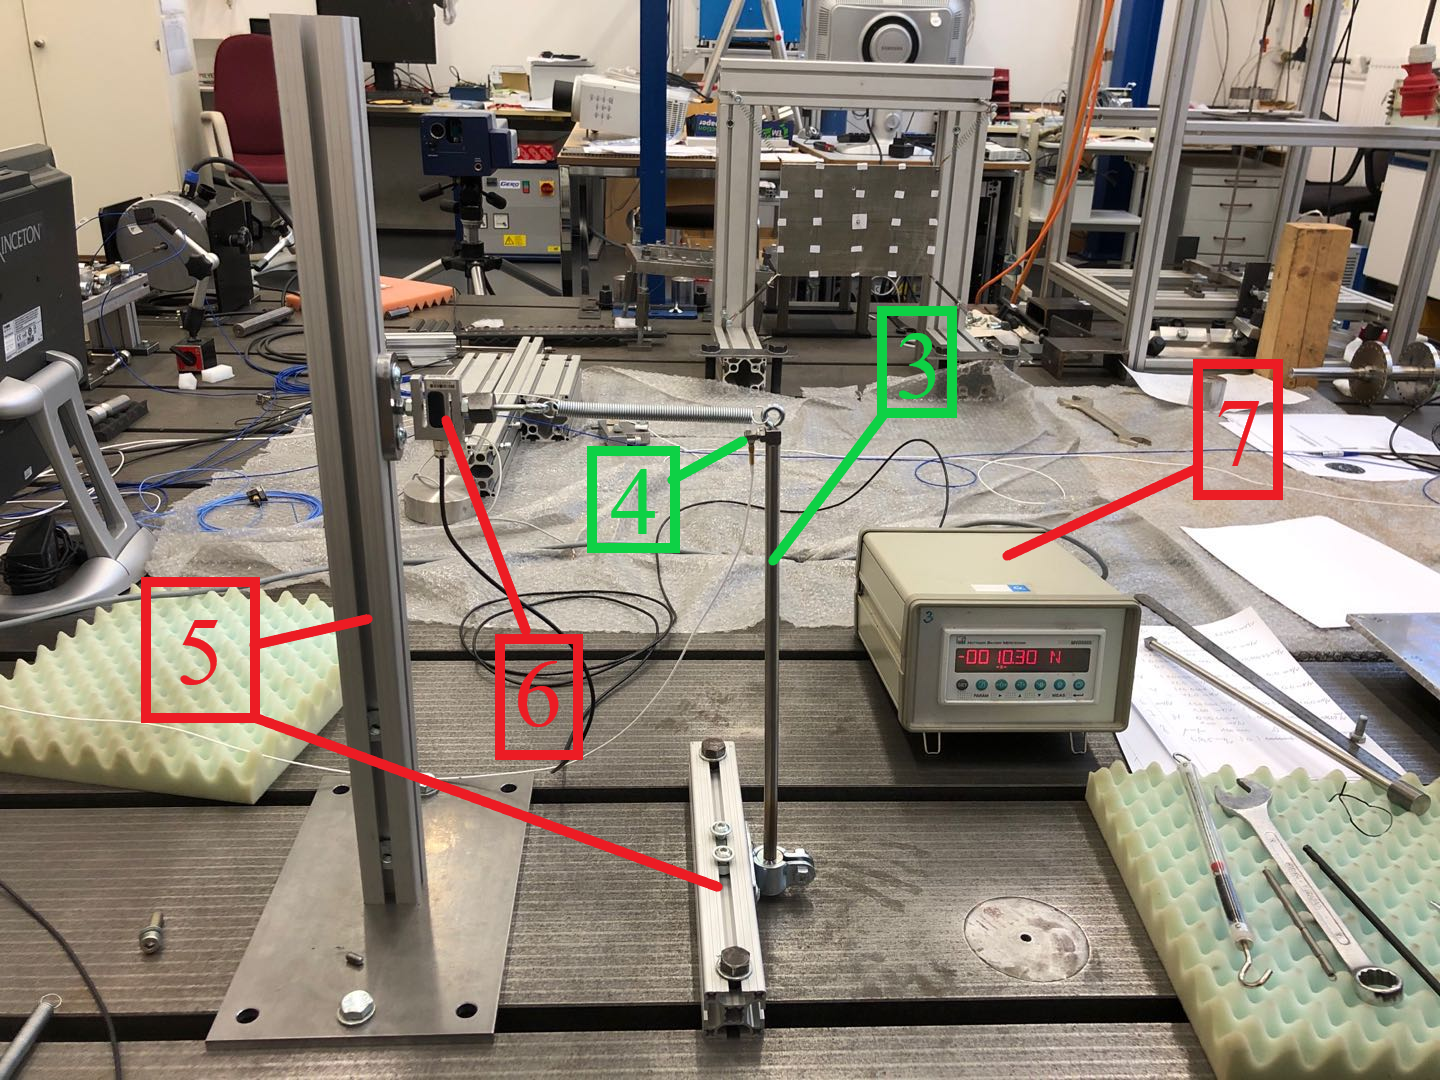
\includegraphics[width=0.48\linewidth, height=0.25\textheight]{Experimentelle_Untersuchungen/Aufbau_Versuchsstand_02.png} }
		\caption{Versuchsaufbau mit einzelnen Objekten.}
		\label{fig:Versuchsaufbau}
	\end{figure}

	
	\subsubsection{Messsoftware}\label{sec:Messsoftware}
	
	In Bezug auf die Messsoftware werden in dieser Arbeit zwei Softwarepakete verwendet. Bei dem ersten handelt es sich um \textsc{PULSE LabShop} von der Firma \textsc{Brüel \& Kj\ae{}r}. Damit werden die Sensorsignale analysiert und für mehrere Messwiederholungen gemittelt. Die für dieses Experiment verwendete Bedienoberfläche von \textsc{PULSE LabShop} ist im Wesentlichen in Abbildung \ref{fig:B&K-Software} dargestellt.
	
	\begin{figure}[H]
		\centering
		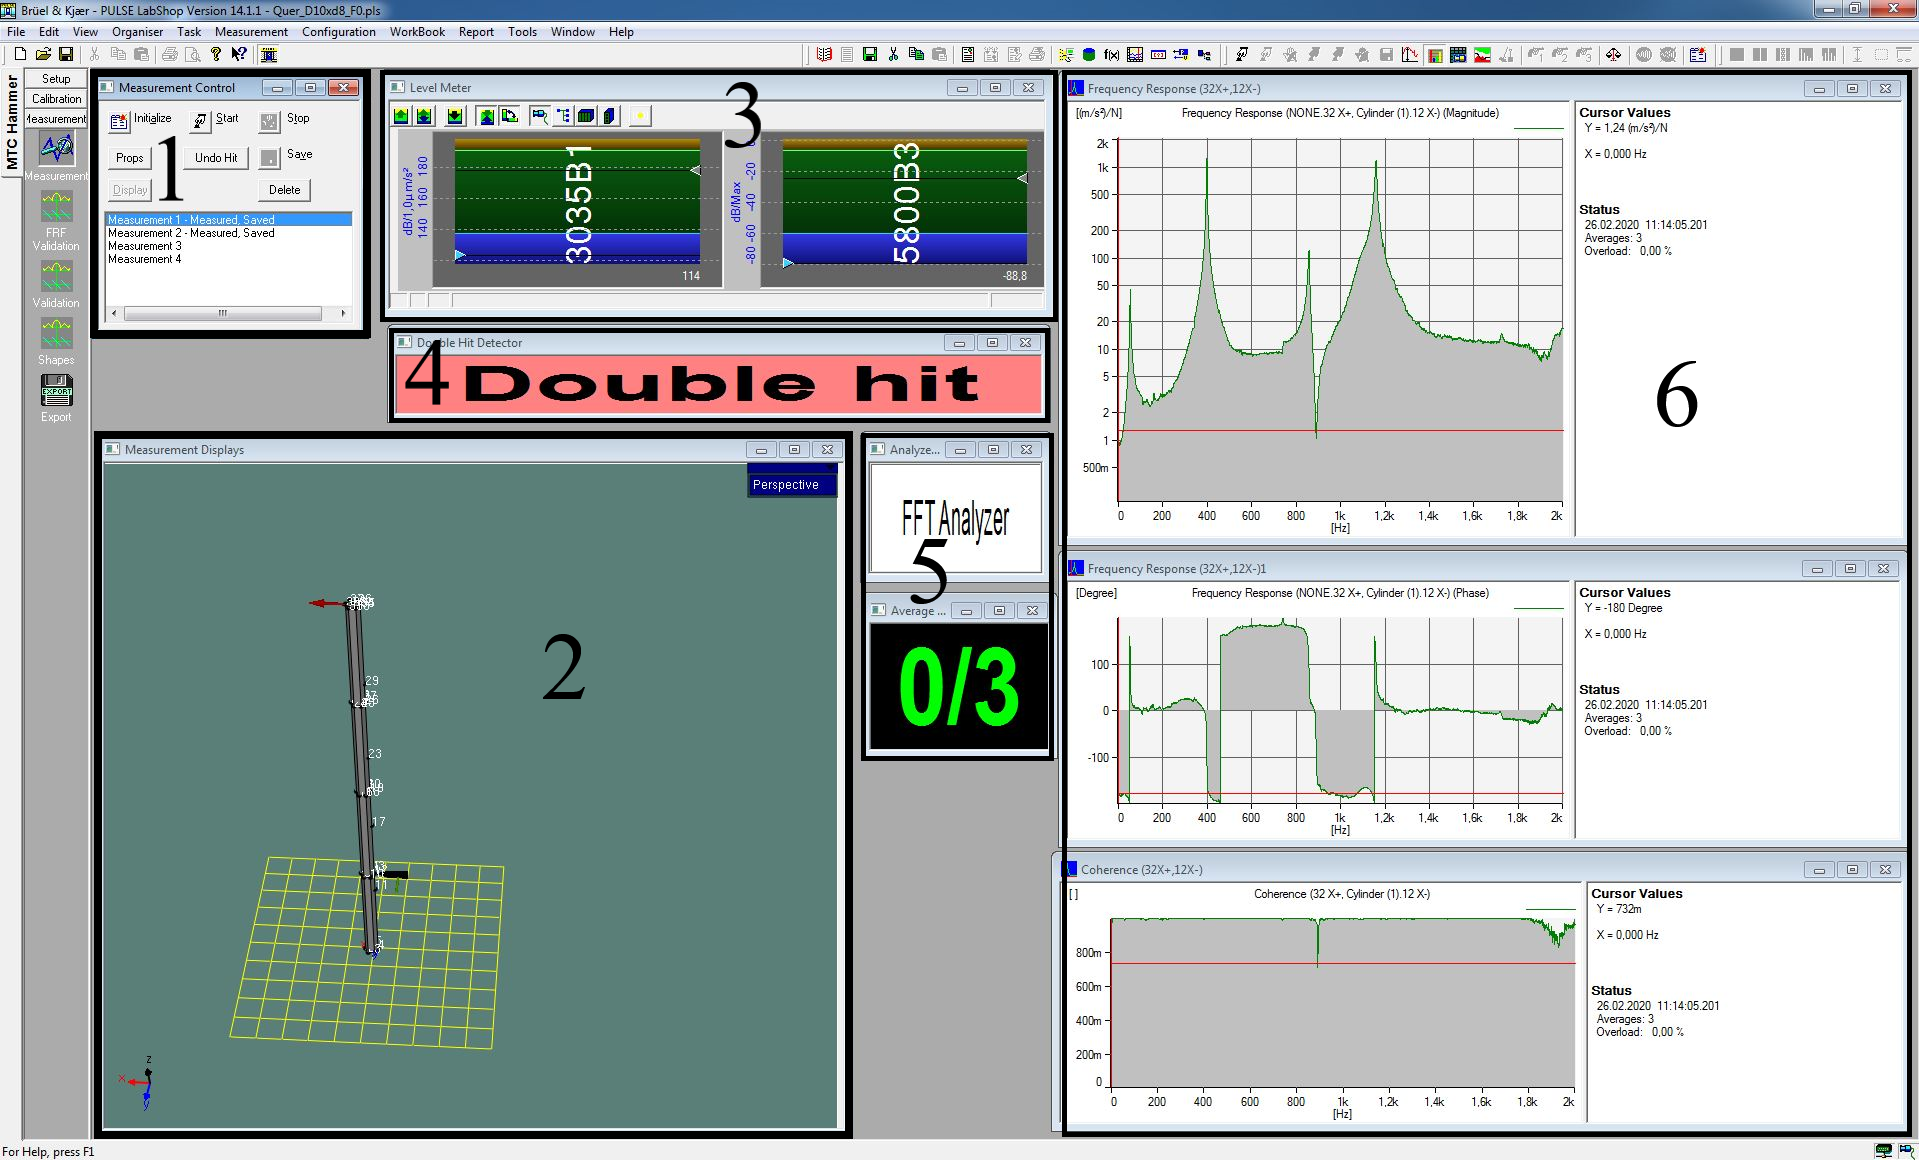
\includegraphics[width=0.96\linewidth, height=0.42\textheight]{Experimentelle_Untersuchungen/Schaft_10x8_0N_parallel_Messung.png}
		\caption{Userinterface für \textsc{PULSE LabShop} Version 14.1.1 von \textsc{Brüel \& Kj\ae{}r}.}
		\label{fig:B&K-Software}
	\end{figure}
	Die einzelnen Bildbereiche besitzen dabei folgende Bedeutung:
	\begin{itemize}
		\item Bereich 1: Steuerung der experimentelle Aktionen, einschließlich Initialisierung, Start, Stopp und Auswahl von Messpunkten. Für jeden Messpunkt werden die Ergebnissse von drei Messungen gemittelt.
		\item Bereich 2: Visualisierung eines dreidimensionales Modells der des Probenkörpers. Angezeigt werden die Punkte der Anregung (schwarzer Pfeil) und der Punkt der Beschleunigungsmessung (roter Pfeil).  und der Anzeige von Messpunkten.
		\item Bereich 3: Anzeige des aktuellen Messpegels für den Kraft und Beschleunigungssensor.
		\item Bereich 4: Mit diesem Erkennungsmodul werden eventuelle Doppelschläge angezeigt.
		\item Bereich 5: Anzeige der erfolgreich durchgeführten Messungen pro Messpunkt. 
		\item Bereich 6: Anzeige der gemessenen Übertragungsfunktion für den aktuellen Messpunkt (oben), Phasenwinkel (mitte) und Kohörenzfunktion (unten).
	\end{itemize}
	
	Es werden die Übertragungsfunktionen für vier Messpunkte am Schaft ermittelt. Mit den drei Wiederholungen je Messpunkt ergeben sich 12 Messungen pro Schaft. Die Weiterverarbeitung der Übertragungsfunktionen erfolgt mit der zweiten Software \textsc{ME'scopeVES} von \textsc{Vibrant Technology Inc.} Damit können die Modalparameter und auch die Modeformen ermittelt werden. Abschließend zeigt Abbildung \ref{fig:ME'scopeVES-Software} das dazugehörige Userinterface.
	
	\begin{figure}[H]
		\centering
		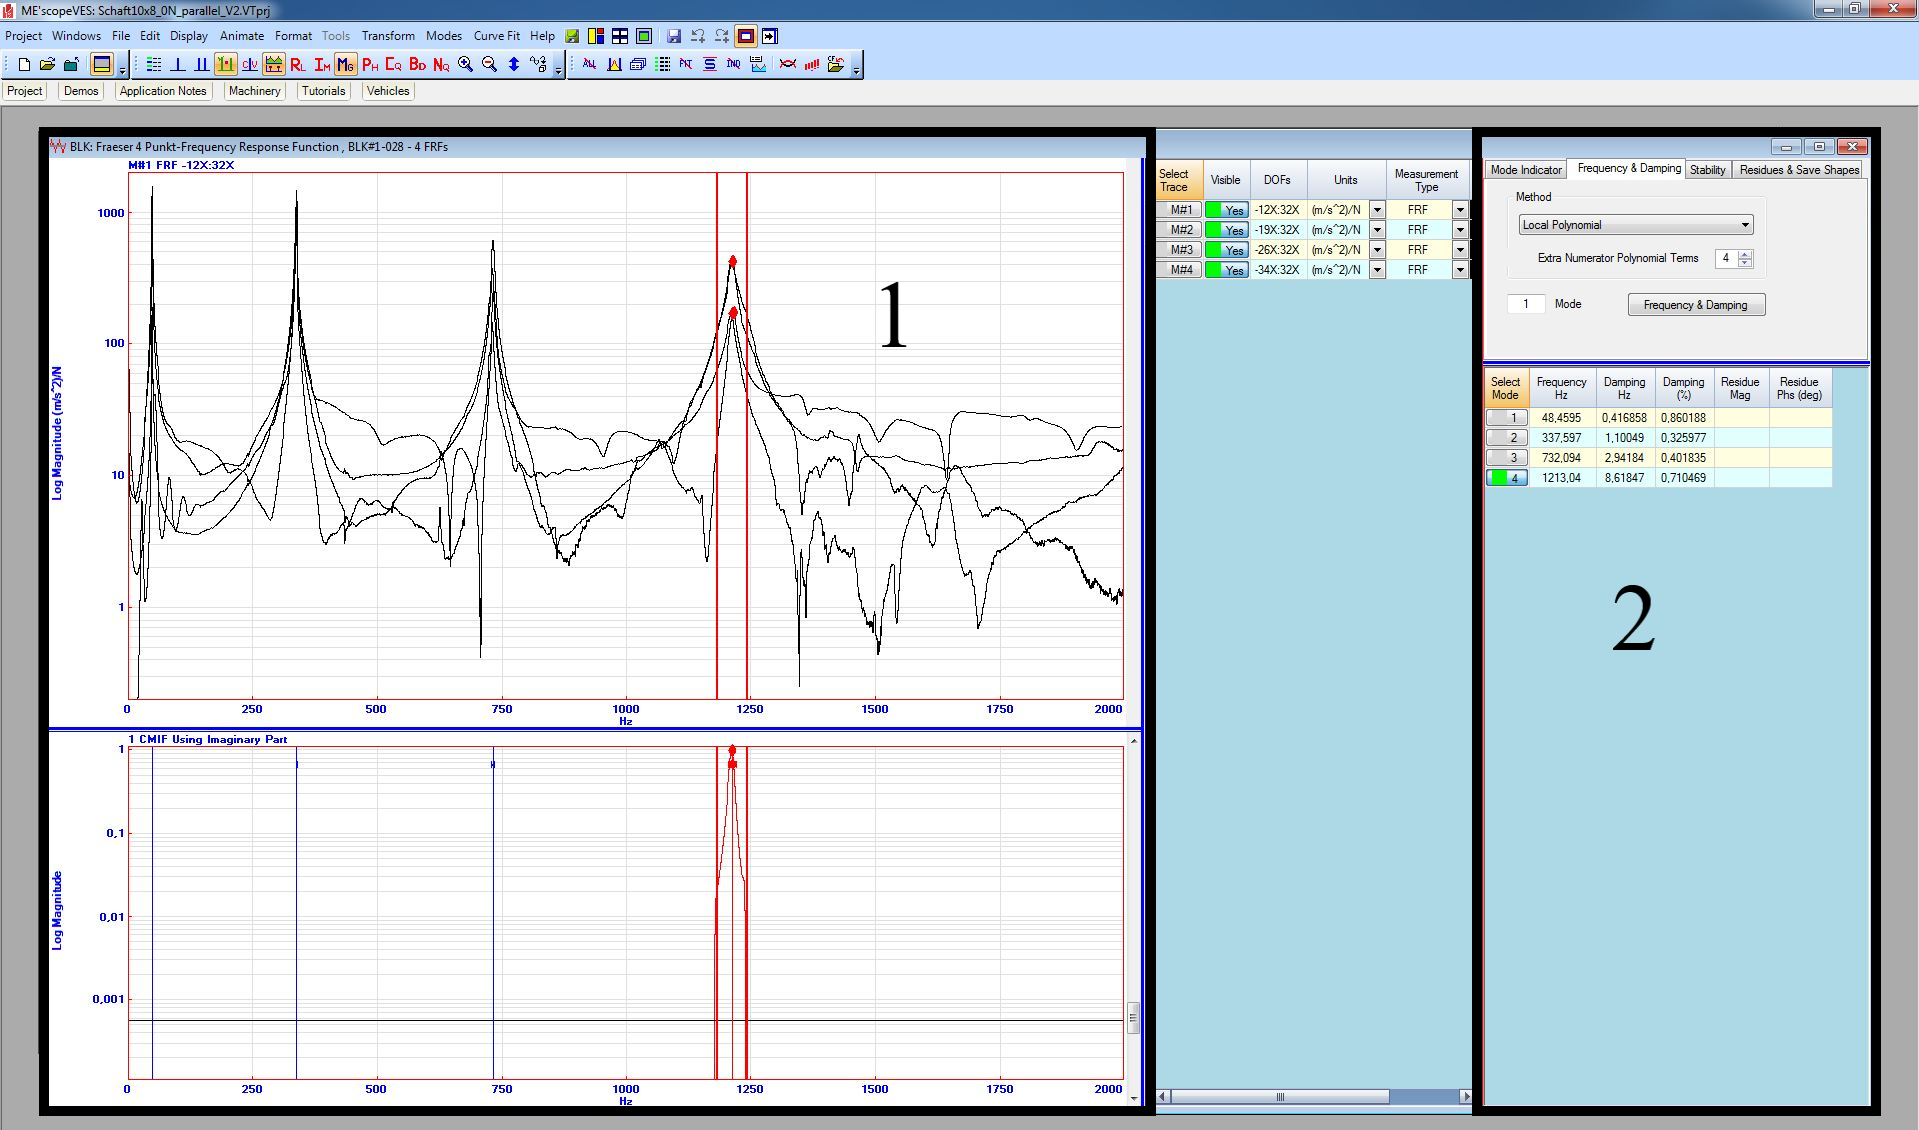
\includegraphics[width=0.97\linewidth, height=0.42\textheight]{Experimentelle_Untersuchungen/Schaft_10x8_0N_parallel_Ergebnisse.png}
		\caption{Userinterface der Software \textsc{ME'scopeVES} von \textsc{Vibrant Technology Inc.}}
		\label{fig:ME'scopeVES-Software}
	\end{figure}
	
	Der Bereich 1 zeigt die vier Übertragungsfunktionen in einem Diagramm. Gut zu erkennen sind die einzelnen Peaks, welche die Eigenfrequenzen darstellen. Im Bereich 2 sind die ermittelten Modalparameter (Frequenz und Dämpfung) für die ersten vier Biegemoden dargestellt.
	
	
	
	\subsection{Experimentelle Modalanalyse}\label{sec:Experimentelle Modalanalyse}
	Wie im Versuchsplan angegeben ist zuerst die experimentelle Identifikation der Modalparameter der Struktur durchzuführen. Die Eigenfrequenzen des Probekörper werden als wichtiger Kennwert durch die experimentelle Modalanalyse bestimmt.\\	
	
	Die Messung der Eigenfrequenz erfolgt nach der sogenannten Impulshammermethode. Der einseitige eingespannte HSC-Schaft wird hierfür an vier Punkten nacheinander angeregt. Beim Anschlagen mit dem Impulshammer (Typ 5800B3 von \textsc{Dytran Instruments}) wird das entstehende Kraftsignal aufgezeichnet. Zeitgleich erfolgt die Messung der Antwort mittels des Beschleunigungssensors (Typ 3035B3 von \textsc{Dytran Instruments}), welcher magnetisch mit dem Versuchskörper verbunden ist.\\
	
	Die vom Beschleunigungsmesser und Impulshammer erhaltenen Signale werden von Messsoftware \textsc{PULSE LabShop} verarbeitet und durch die Übertragungsfunktion dargestellt \cite{dossing1989strukturen}. Durch das Exportieren der Messergebnisse in die Software Modalanalyse-Software \textsc{ME'scopeVES} könne die Modalparameter berechnet werden. Im nächsten Kapitel werden die simulierten Eigenfrequenzen und die experimentellen Ergebnisse ausführlich analysiert und verglichen.
	
	